\documentclass[paper=a4, fontsize=11pt]{article}
\usepackage[utf8]{inputenc}
\usepackage[english,magyar]{babel}
\usepackage{amsmath}
\usepackage{graphicx} 
\usepackage{float}
\usepackage{rotating}
\usepackage{latexsym}
\usepackage{blindtext}
\addtolength{\oddsidemargin}{-.875in}
\addtolength{\evensidemargin}{-.875in}
\addtolength{\textwidth}{1.95in}
\addtolength{\topmargin}{-.9in}
\addtolength{\textheight}{1.6in}


\title{\scshape\Huge Sejtautomaták }
\date{\scshape\Large 2018.05.5.}
\author{\scshape\huge Nagy Péter\\\scshape\huge m07ilf}









\begin{document}
\maketitle
\newpage

 
\tableofcontents
\newpage




\section{Conway élet játék}
A sejtautomaták egyik legismertebbike a John Conway által kifejlesztett életjáték. Ebben a modellben a sejtjeink egy sakktábla szerű terepen helyezkednek el, ahol minden sejtnek nyolc darab szomszédja van. A sejtek két féle álapotban lehetnek, vagy élő vagy halott állapotban. A rendszer diszkrét lépésekben fejlödik és a sejtek müködése a következő:

\begin{itemize}
\item Ha a sejtnek n élő szomszédja van akkor a sejt állapota nem változik
\item Ha n+1 szomszédja van akkor a sejt élő lesz, függetlenül a jelenlegi állapotától
\item Minden más esetben a sejt elpusztul
\end{itemize}


Az életjáték sok összetett rendszer növekedését, csökkenését vagy mozgását tudja szimulálni. 
A szimuláció Turing-teljes vagyis bármit amit kilehet algoritmusokkal számolni azt képes kiszámolni.Conway egyik sejtése az volt, hogy a növekedésnek van egy felső korláta. 1970-ben ötven dolláros jutalmat kínált azért, hogy ezt valakí igazolja vagy cáfolja. A díjat Bill Gosper által vezetett csapata nyerte el a ma már Gosper glider gun nevű mintázattal. Ez egy olyan pisztoly amely tőle elfelé mozgó alakzatokat lő ki.
\\
\\
\\

\begin{figure}[H]
    \centering
    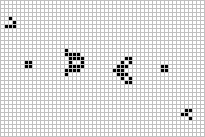
\includegraphics[width=\textwidth]{Gosperglidergun_destruct}
    \caption{Gosper glider gun}
\end{figure}











\newpage
\subsection{Nyílt peremfeltétel}
Első esetben nézzük meg milyen lesz a nyílt határokkal a szimulációt. 
\\
\\
\\
n=1 eset:
\begin{tabular}{cccc}
1&1&1&0\\
0&0&1&0\\
1&1&0&0\\
0&0&1&1
\end{tabular}
\quad
\begin{tabular}{cccc}
1&0&1&1\\
0&0&0&1\\
0&0&0&0\\
1&0&1&1
\end{tabular}
\quad
\begin{tabular}{cccc}
0&1&1&1\\
1&1&0&1\\
0&1&0&0\\
0&1&1&1
\end{tabular}
\quad
\begin{tabular}{cccc}
0&0&0&1\\
1&0&0&1\\
0&0&0&0\\
1&1&0&1
\end{tabular}
\\
\\
\\
n=2 eset:
\begin{tabular}{cccc}
1&1&1&0\\
0&0&1&0\\
1&1&0&0\\
0&0&1&1
\end{tabular}
\quad
\begin{tabular}{cccc}
0&1&1&0\\
0&0&1&0\\
0&1&0&1\\
0&1&1&0
\end{tabular}
\quad
\begin{tabular}{cccc}
0&1&1&0\\
0&0&0&1\\
0&1&0&1\\
0&1&1&0
\end{tabular}
\quad
\begin{tabular}{cccc}
0&0&1&0\\
0&1&0&1\\
0&1&0&1\\
0&1&1&0
\end{tabular}
\\
\\
\\
n=3 eset:
\begin{tabular}{cccc}
1&1&1&0\\
0&0&1&0\\
1&1&0&0\\
0&0&1&1
\end{tabular}
\quad
\begin{tabular}{cccc}
0&1&0&0\\
0&0&1&0\\
0&1&1&0\\
0&0&0&0
\end{tabular}
\quad
\begin{tabular}{cccc}
0&0&0&0\\
0&1&1&0\\
0&0&0&0\\
0&0&0&0
\end{tabular}
\quad
\begin{tabular}{cccc}
0&0&1&0\\
0&0&0&0\\
0&0&0&0\\
0&0&0&0
\end{tabular}
\\
\\
\\
n=4 eset:
\begin{tabular}{cccc}
1&1&1&0\\
0&0&1&0\\
1&1&0&0\\
0&0&1&1
\end{tabular}
\quad
\begin{tabular}{cccc}
0&0&0&0\\
1&0&0&0\\
0&0&0&0\\
0&0&0&0
\end{tabular}
\quad
\begin{tabular}{cccc}
0&0&0&0\\
0&0&0&0\\
0&0&0&0\\
0&0&0&0
\end{tabular}
\quad
\begin{tabular}{cccc}
0&0&0&0\\
0&0&0&0\\
0&0&0&0\\
0&0&0&0
\end{tabular}
\\
\\
\\
n=4 eset:
\begin{tabular}{cccc}
1&1&1&0\\
0&0&1&0\\
1&1&0&0\\
0&0&1&1
\end{tabular}
\quad
\begin{tabular}{cccc}
0&0&0&0\\
0&1&0&0\\
0&0&0&0\\
0&0&0&0
\end{tabular}
\quad
\begin{tabular}{cccc}
0&0&0&0\\
0&0&0&0\\
0&0&0&0\\
0&0&0&0
\end{tabular}
\quad
\begin{tabular}{cccc}
0&0&0&0\\
0&0&0&0\\
0&0&0&0\\
0&0&0&0
\end{tabular}
\\
\\
\\
n=5 eset:
\begin{tabular}{cccc}
1&1&1&0\\
0&0&1&0\\
1&1&0&0\\
0&0&1&1
\end{tabular}
\quad
\begin{tabular}{cccc}
0&0&0&0\\
0&0&0&0\\
0&0&0&0\\
0&0&0&0
\end{tabular}
\quad
\begin{tabular}{cccc}
0&0&0&0\\
0&0&0&0\\
0&0&0&0\\
0&0&0&0
\end{tabular}
\quad
\begin{tabular}{cccc}
0&0&0&0\\
0&0&0&0\\
0&0&0&0\\
0&0&0&0
\end{tabular}








\newpage
\subsection{Élő határ}
Ebben az esetben vizsgáljuk az életjátékot különböző n értékekre úgy, hogy a határon mindenhol élő sejteket feltételezünk.
\\
\\
\\
n=1 eset:
\begin{tabular}{cccc}
0&1&0&1\\
0&0&0&0\\
0&1&1&0\\
1&0&0&1
\end{tabular}
\quad
\begin{tabular}{cccc}
0&0&0&0\\
0&0&0&0\\
0&1&1&0\\
0&0&0&0
\end{tabular}
\quad
\begin{tabular}{cccc}
0&0&0&0\\
0&1&1&0\\
0&1&1&0\\
0&0&0&0
\end{tabular}
\quad
\begin{tabular}{cccc}
0&0&0&0\\
0&0&0&0\\
0&0&0&0\\
0&0&0&0
\end{tabular}
\newline
\\
\\
\\
n=2 eset:
\begin{tabular}{cccc}
0&1&0&1\\
0&0&0&0\\
0&1&1&0\\
1&0&0&1
\end{tabular}
\quad
\begin{tabular}{cccc}
0&1&0&0\\
0&1&0&0\\
0&1&1&0\\
0&0&0&0
\end{tabular}
\quad
\begin{tabular}{cccc}
0&0&0&0\\
0&1&0&0\\
0&1&1&0\\
0&0&0&0
\end{tabular}
\quad
\begin{tabular}{cccc}
0&0&0&0\\
0&0&0&0\\
0&0&0&0\\
0&0&0&0
\end{tabular}
\\
\\
\\
n=3 eset:
\begin{tabular}{cccc}
0&1&0&1\\
0&0&0&0\\
0&1&1&0\\
1&0&0&1
\end{tabular}
\quad
\begin{tabular}{cccc}
0&1&0&0\\
0&0&1&0\\
1&0&0&0\\
0&0&0&0
\end{tabular}
\quad
\begin{tabular}{cccc}
0&1&0&0\\
0&0&0&1\\
1&0&0&1\\
0&1&0&0
\end{tabular}
\quad
\begin{tabular}{cccc}
0&1&0&0\\
0&0&0&1\\
1&0&0&1\\
0&1&0&0
\end{tabular}
\\
\\
\\
n=4 eset:
\begin{tabular}{cccc}
0&1&0&1\\
0&0&0&0\\
0&1&1&0\\
1&0&0&1
\end{tabular}
\quad
\begin{tabular}{cccc}
0&0&1&1\\
1&0&0&1\\
0&0&0&1\\
0&0&0&0
\end{tabular}
\quad
\begin{tabular}{cccc}
0&1&1&0\\
0&0&0&0\\
1&0&0&1\\
1&0&0&0
\end{tabular}
\quad
\begin{tabular}{cccc}
0&1&1&0\\
1&0&0&1\\
1&0&0&0\\
0&1&0&0
\end{tabular}
\\
\\
\\
n=5 eset:
\begin{tabular}{cccc}
0&1&0&1\\
0&0&0&0\\
0&1&1&0\\
1&0&0&1
\end{tabular}
\quad
\begin{tabular}{cccc}
1&0&0&1\\
0&0&0&0\\
0&0&0&0\\
1&1&1&1
\end{tabular}
\quad
\begin{tabular}{cccc}
1&0&0&1\\
0&0&0&0\\
0&0&0&0\\
1&1&1&1
\end{tabular}
\quad
\begin{tabular}{cccc}
1&0&0&1\\
0&0&0&0\\
0&0&0&0\\
1&1&1&1
\end{tabular}
\\
\\
\\
n=6 eset:
\begin{tabular}{cccc}
0&1&0&1\\
0&0&0&0\\
0&1&1&0\\
1&0&0&1
\end{tabular}
\quad
\begin{tabular}{cccc}
0&0&0&0\\
0&0&0&0\\
0&0&0&0\\
1&0&0&1
\end{tabular}
\quad
\begin{tabular}{cccc}
0&0&0&0\\
0&0&0&0\\
0&0&0&0\\
0&0&0&0
\end{tabular}
\quad
\begin{tabular}{cccc}
0&0&0&0\\
0&0&0&0\\
0&0&0&0\\
0&0&0&0
\end{tabular}
\\
\\
\\
n=7 eset:
\begin{tabular}{cccc}
0&1&0&1\\
0&0&0&0\\
0&1&1&0\\
1&0&0&1
\end{tabular}
\quad
\begin{tabular}{cccc}
0&0&0&0\\
0&0&0&0\\
0&0&0&0\\
0&0&0&0
\end{tabular}
\quad
\begin{tabular}{cccc}
0&0&0&0\\
0&0&0&0\\
0&0&0&0\\
0&0&0&0
\end{tabular}
\quad
\begin{tabular}{cccc}
0&0&0&0\\
0&0&0&0\\
0&0&0&0\\
0&0&0&0
\end{tabular}


\newpage
\subsection{Periodikus határ}
Vizsgáljuk meg a rendszert úgy, hogy a határokon periodikusan váltakoznak az élő és holt sejtek.
\\
\\
\\
n=1 eset:
\begin{tabular}{cccc}
0&1&0&0\\
1&0&0&1\\
0&1&0&0\\
0&0&1&1
\end{tabular}
\quad
\begin{tabular}{cccc}
0&0&0&0\\
0&0&0&1\\
0&1&0&0\\
0&0&0&0
\end{tabular}
\quad
\begin{tabular}{cccc}
1&1&1&0\\
0&0&1&1\\
0&0&1&1\\
0&0&1&1
\end{tabular}
\quad
\begin{tabular}{cccc}
0&0&0&0\\
0&0&0&0\\
0&0&0&0\\
0&0&0&0
\end{tabular}
\\
\\
\\
n=2 eset:
\begin{tabular}{cccc}
0&1&0&0\\
1&0&0&1\\
0&1&0&0\\
0&0&1&1
\end{tabular}
\quad
\begin{tabular}{cccc}
0&1&1&0\\
0&1&1&1\\
1&1&0&0\\
0&0&1&1
\end{tabular}
\quad
\begin{tabular}{cccc}
0&0&0&0\\
0&0&0&0\\
1&0&0&0\\
0&0&1&1
\end{tabular}
\quad
\begin{tabular}{cccc}
0&0&0&1\\
1&0&0&0\\
0&0&0&1\\
0&0&1&1
\end{tabular}
\\
\\
\\
n=3 eset:
\begin{tabular}{cccc}
0&1&0&0\\
1&0&0&1\\
0&1&0&0\\
0&0&1&1
\end{tabular}
\quad
\begin{tabular}{cccc}
1&1&0&1\\
1&0&0&0\\
0&0&1&1\\
1&1&1&1
\end{tabular}
\quad
\begin{tabular}{cccc}
1&1&0&1\\
0&1&1&0\\
0&0&1&1\\
1&0&0&0
\end{tabular}
\quad
\begin{tabular}{cccc}
1&0&0&1\\
0&1&0&0\\
0&1&1&1\\
1&1&0&1
\end{tabular}
\\
\\
\\
n=4 eset:
\begin{tabular}{cccc}
0&1&0&0\\
1&0&0&1\\
0&1&0&0\\
0&0&1&1
\end{tabular}
\quad
\begin{tabular}{cccc}
0&0&0&0\\
1&0&0&0\\
0&0&0&0\\
0&0&0&0
\end{tabular}
\quad
\begin{tabular}{cccc}
0&0&0&0\\
0&0&0&0\\
0&0&0&0\\
0&0&0&0
\end{tabular}
\quad
\begin{tabular}{cccc}
0&0&0&0\\
0&0&0&0\\
0&0&0&0\\
0&0&0&0
\end{tabular}
\\
\\
\\
n=5 eset:
\begin{tabular}{cccc}
0&1&0&0\\
1&0&0&1\\
0&1&0&0\\
0&0&1&1
\end{tabular}
\quad
\begin{tabular}{cccc}
0&0&0&0\\
0&0&0&0\\
0&0&0&0\\
0&0&0&0
\end{tabular}
\quad
\begin{tabular}{cccc}
0&0&0&0\\
0&0&0&0\\
0&0&0&0\\
0&0&0&0
\end{tabular}
\quad
\begin{tabular}{cccc}
0&0&0&0\\
0&0&0&0\\
0&0&0&0\\
0&0&0&0
\end{tabular}


\newpage
\subsection{Véletlen eloszlású hatér}
Vizsgáljuk meg a rendszert úgy, hogy a határon véletlen vannak elhelyezve az élő és holt sejtek.
\\
\\
\\
n=1 eset:
\begin{tabular}{cccc}
0&1&0&1\\
1&0&0&1\\
0&1&0&0\\
1&0&0&1
\end{tabular}
\quad
\begin{tabular}{cccc}
0&1&0&1\\
1&0&0&0\\
0&1&0&0\\
1&1&0&1
\end{tabular}
\quad
\begin{tabular}{cccc}
0&1&1&0\\
0&0&0&0\\
0&0&0&0\\
0&0&0&0
\end{tabular}
\quad
\begin{tabular}{cccc}
0&0&1&0\\
1&1&1&0\\
0&0&0&1\\
0&0&1&0
\end{tabular}
\\
\\
\\
n=2 eset:
\begin{tabular}{cccc}
0&1&0&1\\
1&0&0&1\\
0&1&0&0\\
1&0&0&1
\end{tabular}
\quad
\begin{tabular}{cccc}
0&1&1&0\\
1&1&0&1\\
0&1&1&1\\
1&0&0&0
\end{tabular}
\quad
\begin{tabular}{cccc}
0&1&0&0\\
1&0&0&1\\
0&0&0&1\\
0&0&0&0
\end{tabular}
\quad
\begin{tabular}{cccc}
0&1&0&1\\
0&0&1&1\\
1&0&0&1\\
1&0&0&0
\end{tabular}
\\
\\
\\
n=3 eset:
\begin{tabular}{cccc}
0&1&0&1\\
1&0&0&1\\
0&1&0&0\\
1&0&0&1
\end{tabular}
\quad
\begin{tabular}{cccc}
1&0&0&1\\
1&0&1&1\\
0&0&0&0\\
0&0&0&0
\end{tabular}
\quad
\begin{tabular}{cccc}
1&0&1&0\\
1&0&0&0\\
1&0&0&0\\
0&0&0&0
\end{tabular}
\quad
\begin{tabular}{cccc}
0&0&0&0\\
0&1&0&0\\
0&0&0&0\\
0&0&0&0
\end{tabular}
\\
\\
\\
n=4 eset:
\begin{tabular}{cccc}
0&1&0&1\\
1&0&0&1\\
0&1&0&0\\
1&0&0&1
\end{tabular}
\quad
\begin{tabular}{cccc}
1&0&0&0\\
1&0&0&0\\
1&0&0&0\\
0&0&0&0
\end{tabular}
\quad
\begin{tabular}{cccc}
0&0&0&0\\
0&0&0&0\\
0&0&0&0\\
0&0&0&0
\end{tabular}
\quad
\begin{tabular}{cccc}
0&0&0&0\\
0&0&0&0\\
0&0&0&0\\
0&0&0&0
\end{tabular}
\\
\\
\\
n=5 eset:
\begin{tabular}{cccc}
0&1&0&1\\
1&0&0&1\\
0&1&0&0\\
1&0&0&1
\end{tabular}
\quad
\begin{tabular}{cccc}
0&0&0&0\\
0&0&0&0\\
0&0&0&0\\
0&0&0&0
\end{tabular}
\quad
\begin{tabular}{cccc}
0&0&0&0\\
0&0&0&0\\
0&0&0&0\\
0&0&0&0
\end{tabular}
\quad
\begin{tabular}{cccc}
0&0&0&0\\
0&0&0&0\\
0&0&0&0\\
0&0&0&0
\end{tabular}





\newpage
\section{Két dimenziós homokdomb modell}


A két dimenziós homokdomb modell a P. Bak, C. Tang and K. Wiesenfeld, Phys. Rev. Lett. 59, 381 (1987) cikkben lett bemutatva. Ennek a modellnek különböző csúcsai vannak, amelyeket egy skalár értékkel lehet jelemezni. Ha ez a skalár értéke nagyobb, mint három akkor a csúcs instabil. Egy ciklusban a homokdomb modell a következő képpen frissül:
\begin{itemize}
\item ha $s_{ij}>3$ ekkor eltávolitunk négy egységet a csúcsról és a szomszédos csúcsokra átteszünk egyet egyet. 
\item ez addig ismétlödik mindenhol amíg el nem érünk egy stabil állapotba
\end{itemize}










\begin{figure}[H]
    \centering
    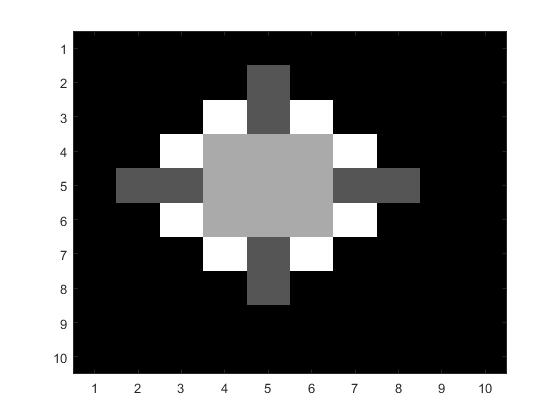
\includegraphics[width=0.65\textwidth]{homok}
    \caption{középre ejtett homok szemek}
\end{figure}










\begin{figure}[H]
    \centering
    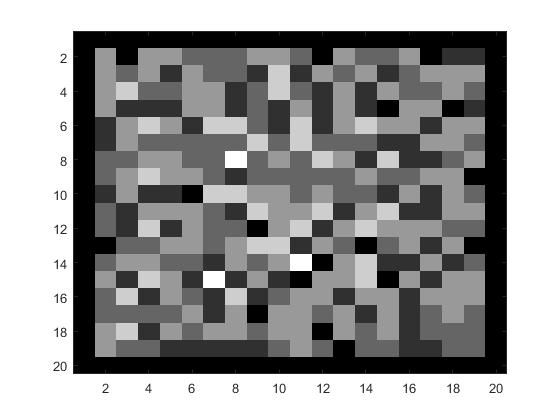
\includegraphics[width=0.65\textwidth]{randomhomok}
    \caption{véletlenül elszórt homok szemek}
\end{figure}


Legyen $n_t$ a felborulások száma a lavinában. Azáltal, hogy nagy számú lavinát generálunk megtudjuk mérni az eloszlását a lavinák számának a borulások számának a függvényében.
\newline
Ilyenkor a modellnek hatvány törvényes viselkedése van:
\begin{align}
N(n_t)\sim \frac{1}{n_t^b}
\end{align}
Itt a b a hatvány törvény kitevője.
\\
\\
Ebből az következik, hogy a lavináknak nincsen természetes méretük vagy skálájuk. Ha b értéke nagyon kicsi akkor minden féle folyamat azonos valószinüséggel tud lejátszódni, ha b értéke nagyobb, mint nulla akkor a nagy események inkább törénnek meg mint a kicsik. A különleges tulajdonsága a hatványtörvénynek, hogy a különböző méretű események hányadosa egy rögzitett szorzó érték lesz ami független az esemény méretétől. Ha szorzó 10 akkor például így fog alakulni:
\begin{align}
\frac{N(10n_t)}{N(n_t)}=\frac{1}{10^b}
\end{align}
Ebben az esetben a homokdomb modellre a b értéke körülbelül 1 lesz.




\begin{figure}[H]
    \centering
    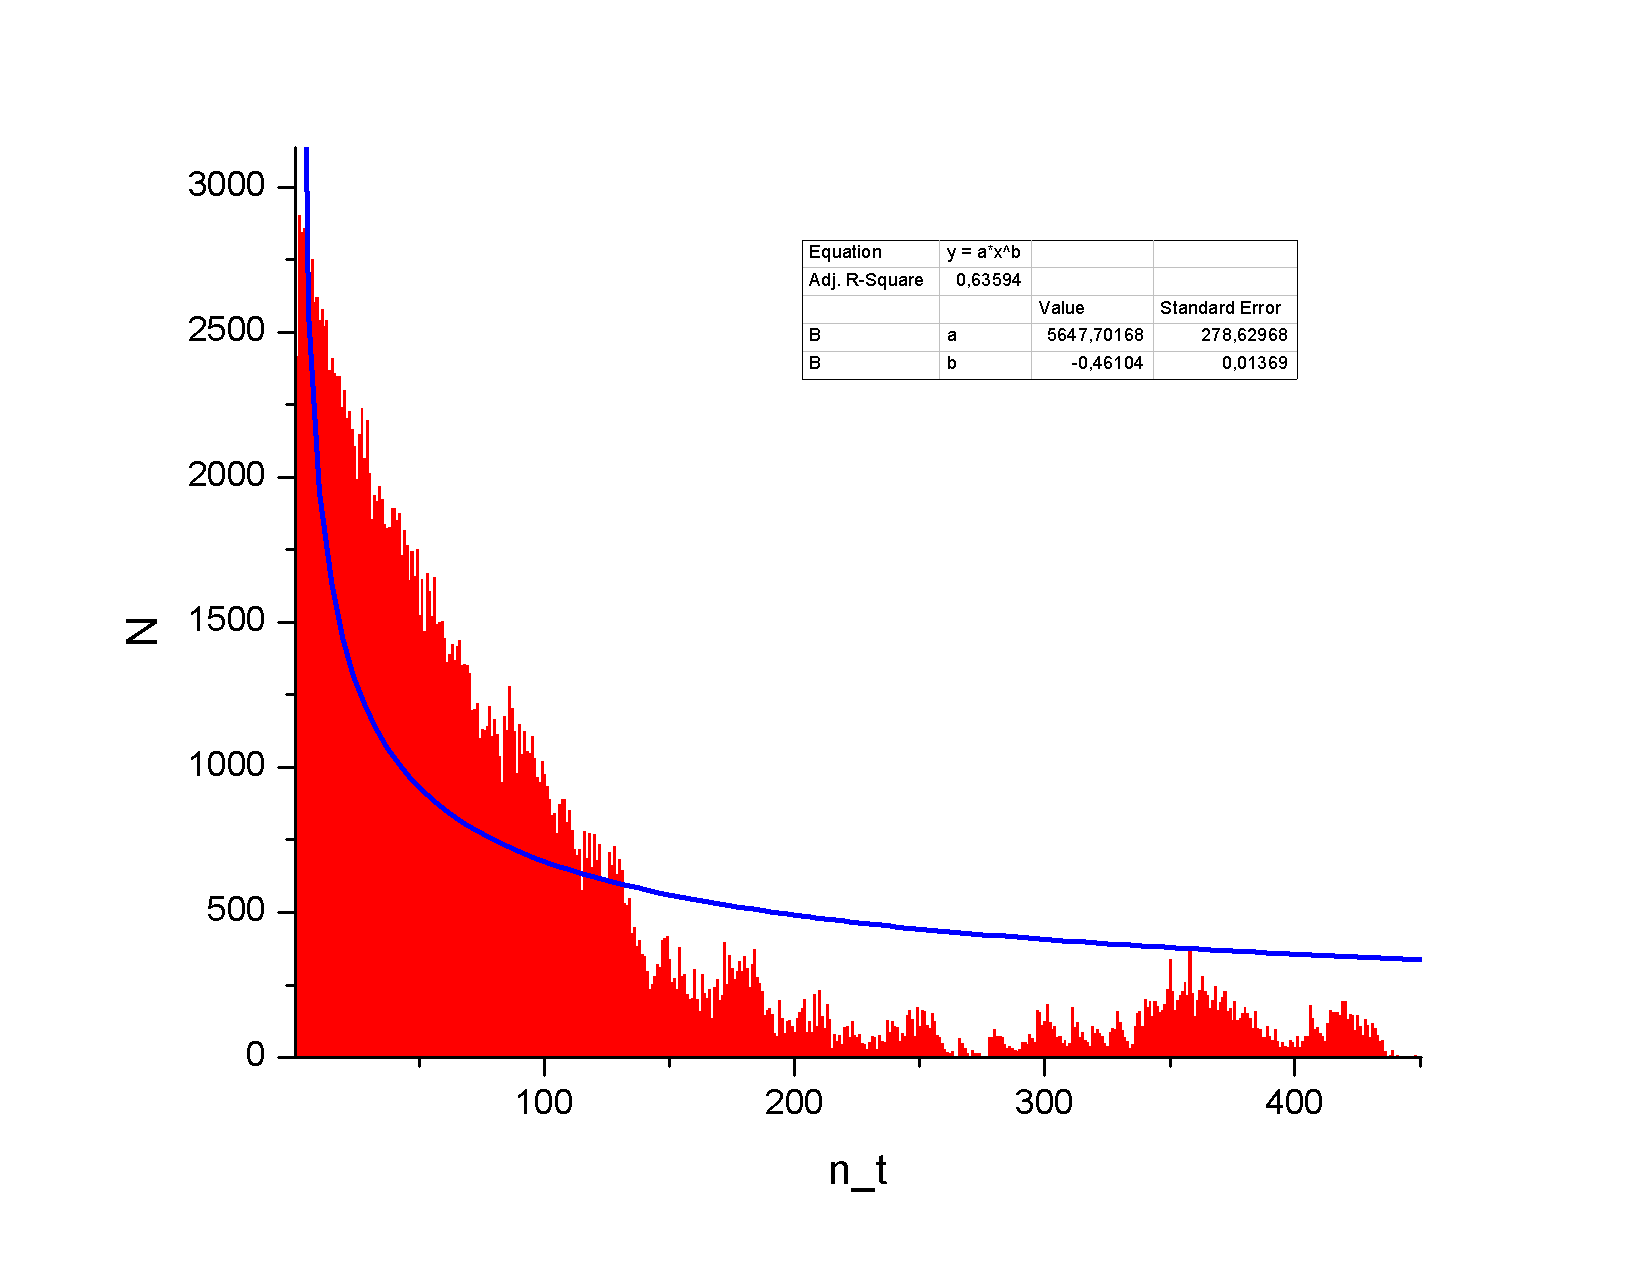
\includegraphics[width=\textwidth]{power}
    \caption{A powe-law függvény }
\end{figure}


































\newpage
\section{Függelék}
\subsection{Conway élet játék nyílt peremfeltétel}
\begin{verbatim}
#include <fstream>
#include <algorithm>
#include <iostream>
#include <cmath>
#include <string>
#include <sstream>
using namespace std;


int main(int argc, char **argv)
{
string matrix_file;
unsigned int N = atoi(argv[2]); 
unsigned int M = atoi(argv[1]); 
matrix_file = argv[3];
int n;
cout<< "Add meg n erteket: ";
cin >> n;
ifstream Mat_file(matrix_file.c_str());
int **matrix = new int*[M];
for ( unsigned int i=0; i<M; i++)
{
matrix[i] = new int[N];
}
int **temp_matrix = new int*[M];
for ( unsigned int i=0; i<M; i++)
{
temp_matrix[i] = new int[N];
}
for ( unsigned int m=0; m<M ; m++)
{
for ( unsigned int n=0; n<N ; n++)
{
Mat_file >> matrix[m][n];
temp_matrix[m][n]=matrix[m][n];
}
}
Mat_file.close();
unsigned int suma; 
for ( unsigned int i=0; i<10 ; i++)
{
ostringstream file;
file << i << ".dat";
ofstream result(file.str().c_str());
for ( unsigned int k=0; k<M; k++)
{
for ( unsigned int j=0; j<N; j++)
{
//határfeltételek
if (k==0 && j==0)
{
suma=matrix[k+1][j]+matrix[k+1][j+1]+matrix[k][j+1];
}
else if (k==(M-1) && j==(N-1))
{
suma=matrix[k-1][j]+matrix[k-1][j-1]+matrix[k][j-1];
}
else if (k==0 && j==(N-1))
{
suma=matrix[k+1][j]+matrix[k+1][j-1]+matrix[k][j-1];
}
else if (k==(M-1) && j==0)
{
suma=matrix[k-1][j]+matrix[k][j+1]+matrix[k-1][j+1];
}
else if (k==0)
{
suma=matrix[k+1][j+1]+matrix[k+1][j-1]+matrix[k+1][j]+matrix[k][j-1]+matrix[k][j+1];
}
else if (k==(M-1))
{
suma=matrix[k-1][j+1]+matrix[k-1][j-1]+matrix[k-1][j]+matrix[k][j-1]+matrix[k][j+1];
}
else if (j==0)
{
suma=matrix[k-1][j]+matrix[k+1][j]+matrix[k-1][j+1]+matrix[k+1][j+1]+matrix[k-1][j];
}
else if (j==(N-1))
{
suma=matrix[k-1][j]+matrix[k+1][j]+matrix[k+1][j-1]+matrix[k-1][j-1]+matrix[k][j-1];
}
else
{
suma=matrix[k-1][j-1]+matrix[k-1][j]+matrix[k-1][j+1]+matrix[k][j-1]+matrix[k][j+1]+matrix[k+1][j-1]+matrix[k+1][j]+matrix[k+1][j+1];
}
//lépés
if(suma==(n+1))
temp_matrix[k][j]=1;
if(suma==n)
temp_matrix[k][j]=matrix[k][j];
if(suma>(n+1) || suma<n)
temp_matrix[k][j]=0;
}
}
for ( unsigned int m=0; m<M ; m++)
{
for ( unsigned int n=0; n<N ; n++)
{
result << temp_matrix[m][n] << "\t";
matrix[m][n]=temp_matrix[m][n];
}
result << endl;
}
}
for(int i=0; i<N; ++i)
{
delete[] matrix[i];
}
delete[] matrix;
for(int i=0; i<N; ++i)
{
delete[] temp_matrix[i];
}
delete[] temp_matrix;
return 0;
}
\end{verbatim}


\subsection{Conway élő határ}
\begin{verbatim}
#include <fstream>
#include <algorithm>
#include <iostream>
#include <cmath>
#include <string>
#include <sstream>
using namespace std;


int main(int argc, char **argv)
{
string matrix_file;
unsigned int N = atoi(argv[2]); 
unsigned int M = atoi(argv[1]); 
matrix_file = argv[3];
int n;
cout<< "Add meg n erteket: ";
cin >> n;
ifstream Mat_file(matrix_file.c_str());
int **matrix = new int*[M];
for ( unsigned int i=0; i<M; i++)
{
matrix[i] = new int[N];
}
int **temp_matrix = new int*[M];
for ( unsigned int i=0; i<M; i++)
{
temp_matrix[i] = new int[N];
}
for ( unsigned int m=0; m<M ; m++)
{
for ( unsigned int n=0; n<N ; n++)
{
Mat_file >> matrix[m][n];
temp_matrix[m][n]=matrix[m][n];
}
}
Mat_file.close();
unsigned int suma; 
for ( unsigned int i=0; i<10 ; i++)
{
ostringstream file;
file << i << ".dat";
ofstream result(file.str().c_str());
for ( unsigned int k=0; k<M; k++)
{
for ( unsigned int j=0; j<N; j++)
{
//határfeltételek
if (k==0 && j==0)
{
suma=matrix[k+1][j]+matrix[k+1][j+1]+matrix[k][j+1]+5;
}
else if (k==(M-1) && j==(N-1))
{
suma=matrix[k-1][j]+matrix[k-1][j-1]+matrix[k][j-1]+5;
}
else if (k==0 && j==(N-1))
{
suma=matrix[k+1][j]+matrix[k+1][j-1]+matrix[k][j-1]+5;
}
else if (k==(M-1) && j==0)
{
suma=matrix[k-1][j]+matrix[k][j+1]+matrix[k-1][j+1]+5;
}
else if (k==0)
{
suma=matrix[k+1][j+1]+matrix[k+1][j-1]+matrix[k+1][j]+matrix[k][j-1]+matrix[k][j+1]+3;
}
else if (k==(M-1))
{
suma=matrix[k-1][j+1]+matrix[k-1][j-1]+matrix[k-1][j]+matrix[k][j-1]+matrix[k][j+1]+3;
}
else if (j==0)
{
suma=matrix[k-1][j]+matrix[k+1][j]+matrix[k-1][j+1]+matrix[k+1][j+1]+matrix[k-1][j]+3;
}
else if (j==(N-1))
{
suma=matrix[k-1][j]+matrix[k+1][j]+matrix[k+1][j-1]+matrix[k-1][j-1]+matrix[k][j-1]+3;
}
else
{
suma=matrix[k-1][j-1]+matrix[k-1][j]+matrix[k-1][j+1]+matrix[k][j-1]+matrix[k][j+1]+matrix[k+1][j-1]+matrix[k+1][j]+matrix[k+1][j+1];
}
//lépés
if(suma==(n+1))
temp_matrix[k][j]=1;
if(suma==n)
temp_matrix[k][j]=matrix[k][j];
if(suma>(n+1) || suma<n)
temp_matrix[k][j]=0;
}
}
for ( unsigned int m=0; m<M ; m++)
{
for ( unsigned int n=0; n<N ; n++)
{
result << temp_matrix[m][n] << "\t";
matrix[m][n]=temp_matrix[m][n];
}
result << endl;
}
}
for(int i=0; i<N; ++i)
{
delete[] matrix[i];
}
delete[] matrix;
for(int i=0; i<N; ++i)
{
delete[] temp_matrix[i];
}
delete[] temp_matrix;
return 0;
}
\end{verbatim}

\subsection{Conway véletlen generált határ}
\begin{verbatim}
#include <fstream>
#include <algorithm>
#include <iostream>
#include <cmath>
#include <string>
#include <sstream>
#include <random> 
using namespace std;



int veletlen() {
	std::random_device rd;
	std::mt19937 Generator(rd());
	std::uniform_real_distribution<double> Distribution(0, 5);
	return Distribution(Generator);
}

int veletlen2() {
	std::random_device rd;
	std::mt19937 Generator(rd());
	std::uniform_real_distribution<double> Distribution(0, 3);
	return Distribution(Generator);
}



int main(int argc, char **argv)
{
string matrix_file;
unsigned int N = atoi(argv[2]); 
unsigned int M = atoi(argv[1]); 
matrix_file = argv[3];
int n;
cout<< "Add meg n erteket: ";
cin >> n;
ifstream Mat_file(matrix_file.c_str());
int **matrix = new int*[M];
for ( unsigned int i=0; i<M; i++)
{
matrix[i] = new int[N];
}
int **temp_matrix = new int*[M];
for ( unsigned int i=0; i<M; i++)
{
temp_matrix[i] = new int[N];
}
for ( unsigned int m=0; m<M ; m++)
{
for ( unsigned int n=0; n<N ; n++)
{
Mat_file >> matrix[m][n];
temp_matrix[m][n]=matrix[m][n];
}
}
Mat_file.close();
unsigned int suma; 
for ( unsigned int i=0; i<10 ; i++)
{
ostringstream file;
file << i << ".dat";
ofstream result(file.str().c_str());
for ( unsigned int k=0; k<M; k++)
{
for ( unsigned int j=0; j<N; j++)
{
//határfeltételek
if (k==0 && j==0)
{
suma=matrix[k+1][j]+matrix[k+1][j+1]+matrix[k][j+1]+veletlen();
}
else if (k==(M-1) && j==(N-1))
{
suma=matrix[k-1][j]+matrix[k-1][j-1]+matrix[k][j-1]+veletlen();
}
else if (k==0 && j==(N-1))
{
suma=matrix[k+1][j]+matrix[k+1][j-1]+matrix[k][j-1]+veletlen();
}
else if (k==(M-1) && j==0)
{
suma=matrix[k-1][j]+matrix[k][j+1]+matrix[k-1][j+1]+veletlen();
}
else if (k==0)
{
suma=matrix[k+1][j+1]+matrix[k+1][j-1]+matrix[k+1][j]+matrix[k][j-1]+matrix[k][j+1]+veletlen2();
}
else if (k==(M-1))
{
suma=matrix[k-1][j+1]+matrix[k-1][j-1]+matrix[k-1][j]+matrix[k][j-1]+matrix[k][j+1]+veletlen2();
}
else if (j==0)
{
suma=matrix[k-1][j]+matrix[k+1][j]+matrix[k-1][j+1]+matrix[k+1][j+1]+matrix[k-1][j]+veletlen2();
}
else if (j==(N-1))
{
suma=matrix[k-1][j]+matrix[k+1][j]+matrix[k+1][j-1]+matrix[k-1][j-1]+matrix[k][j-1]+veletlen2();
}
else
{
suma=matrix[k-1][j-1]+matrix[k-1][j]+matrix[k-1][j+1]+matrix[k][j-1]+matrix[k][j+1]+matrix[k+1][j-1]+matrix[k+1][j]+matrix[k+1][j+1];
}
//lépés
if(suma==(n+1))
temp_matrix[k][j]=1;
if(suma==n)
temp_matrix[k][j]=matrix[k][j];
if(suma>(n+1) || suma<n)
temp_matrix[k][j]=0;
}
}
for ( unsigned int m=0; m<M ; m++)
{
for ( unsigned int n=0; n<N ; n++)
{
result << temp_matrix[m][n] << "\t";
matrix[m][n]=temp_matrix[m][n];
}
result << endl;
}
}
for(int i=0; i<N; ++i)
{
delete[] matrix[i];
}
delete[] matrix;
for(int i=0; i<N; ++i)
{
delete[] temp_matrix[i];
}
delete[] temp_matrix;
return 0;
}
\end{verbatim}

\subsection{Conway periodikus határ}
\begin{verbatim}
#include <fstream>
#include <algorithm>
#include <iostream>
#include <cmath>
#include <string>
#include <sstream>
using namespace std;


int main(int argc, char **argv)
{
string matrix_file;
unsigned int N = atoi(argv[2]); 
unsigned int M = atoi(argv[1]); 
matrix_file = argv[3];
int n;
cout<< "Add meg n erteket: ";
cin >> n;
ifstream Mat_file(matrix_file.c_str());
int **matrix = new int*[M];
for ( unsigned int i=0; i<M; i++)
{
matrix[i] = new int[N];
}
int **temp_matrix = new int*[M];
for ( unsigned int i=0; i<M; i++)
{
temp_matrix[i] = new int[N];
}
for ( unsigned int m=0; m<M ; m++)
{
for ( unsigned int n=0; n<N ; n++)
{
Mat_file >> matrix[m][n];
temp_matrix[m][n]=matrix[m][n];
}
}
Mat_file.close();
unsigned int suma; 
for ( unsigned int i=0; i<10 ; i++)
{
ostringstream file;
file << i << ".dat";
ofstream result(file.str().c_str());
for ( unsigned int k=0; k<M; k++)
{
for ( unsigned int j=0; j<N; j++)
{


//határfeltételek a sarkakon
if (k==0 && j==0)
{
suma=matrix[k+1][j]+matrix[k+1][j+1]+matrix[k][j+1]+2;
}
else if (k==(M-1) && j==(N-1))
{
suma=matrix[k-1][j]+matrix[k-1][j-1]+matrix[k][j-1]+2;
}
else if (k==0 && j==(N-1))
{
suma=matrix[k+1][j]+matrix[k+1][j-1]+matrix[k][j-1]+3;
}
else if (k==(M-1) && j==0)
{
suma=matrix[k-1][j]+matrix[k][j+1]+matrix[k-1][j+1]+3;
}




//határfeltételek a széleken
else if (k==0 && j%2==!0)
{
suma=matrix[k+1][j+1]+matrix[k+1][j-1]+matrix[k+1][j]+matrix[k][j-1]+matrix[k][j+1]+2;
}
else if (k==0 && j%2==0)
{
suma=matrix[k+1][j+1]+matrix[k+1][j-1]+matrix[k+1][j]+matrix[k][j-1]+matrix[k][j+1]+1;
}
else if (k==(M-1) && j%2==!0)
{
suma=matrix[k-1][j+1]+matrix[k-1][j-1]+matrix[k-1][j]+matrix[k][j-1]+matrix[k][j+1]+2;
}
else if (k==(M-1) && j%2==0)
{
suma=matrix[k-1][j+1]+matrix[k-1][j-1]+matrix[k-1][j]+matrix[k][j-1]+matrix[k][j+1]+1;
}
else if (j==0 && k%2==!0)
{
suma=matrix[k-1][j]+matrix[k+1][j]+matrix[k-1][j+1]+matrix[k+1][j+1]+matrix[k-1][j]+2;
}
else if (j==0 && k%2==0)
{
suma=matrix[k-1][j]+matrix[k+1][j]+matrix[k-1][j+1]+matrix[k+1][j+1]+matrix[k-1][j]+1;
}
else if (j==(N-1) && k%2==!0)
{
suma=matrix[k-1][j]+matrix[k+1][j]+matrix[k+1][j-1]+matrix[k-1][j-1]+matrix[k][j-1]+2;
}
else if (j==(N-1) && k%2==0)
{
suma=matrix[k-1][j]+matrix[k+1][j]+matrix[k+1][j-1]+matrix[k-1][j-1]+matrix[k][j-1]+1;
}

//amugy meg 
else
{
suma=matrix[k-1][j-1]+matrix[k-1][j]+matrix[k-1][j+1]+matrix[k][j-1]+matrix[k][j+1]+matrix[k+1][j-1]+matrix[k+1][j]+matrix[k+1][j+1];
}


//lépés
if(suma==(n+1))
temp_matrix[k][j]=1;
if(suma==n)
temp_matrix[k][j]=matrix[k][j];
if(suma>(n+1) || suma<n)
temp_matrix[k][j]=0;
}
}
for ( unsigned int m=0; m<M ; m++)
{
for ( unsigned int n=0; n<N ; n++)
{
result << temp_matrix[m][n] << "\t";
matrix[m][n]=temp_matrix[m][n];
}
result << endl;
}
}
for(int i=0; i<N; ++i)
{
delete[] matrix[i];
}
delete[] matrix;
for(int i=0; i<N; ++i)
{
delete[] temp_matrix[i];
}
delete[] temp_matrix;
return 0;
}
\end{verbatim}


\subsection{2D homokdomb (Matlab)}
\begin{verbatim}
function [n_t]= homokdomb(N,i)
n_t=zeros(i,1);
In=zeros(N);
[m ,n]=size(In);
figure;
colormap(gray);
imagesc(In);
f = getframe;
[im,map] = rgb2ind(f.cdata,256,'nodither');
pause(5)
for kor=1:i
In(m/2,n/2)=In(m/2,n/2)+1;
for k=2:m-1
for j=2:n-1
if In(k,j)>=4
In(k+1,j)=In(k+1,j)+1;
In(k-1,j)=In(k-1,j)+1;
In(k,j+1)=In(k,j+1)+1;
In(k,j-1)=In(k,j-1)+1;
In(k,j)=In(k,j)-4;
n_t(kor)=n_t(kor)+4;
end
end
end
In(1,:)=0;
In(:,1)=0;
In(n,:)=0;
In(:,n)=0;
imagesc(In)
f = getframe;
im(:,:,1,kor) = rgb2ind(f.cdata,map,'nodither');
pause(0.01)
end
imwrite(im,map,'animation.gif','DelayTime',0.01,'LoopCount',inf)
end
\end{verbatim}


\subsection{2D homokdomb véletlen helyre dobott homokszemekkel (Matlab)}
\begin{verbatim}
function [n_t]=veletlenhomokdomb(N,i)
n_t=zeros(i,1);
In=randi(7,N);
[m, n]=size(In);
figure;
colormap(gray);
imagesc(In);
f = getframe;
[im,map] = rgb2ind(f.cdata,256,'nodither');
pause(5)
for kor=1:i
m_rand=randi(n,1);
n_rand=randi(n,1);
In(m_rand,n_rand)=In(m_rand,n_rand)+1;
for k=2:m-1
for j=2:n-1
if In(k,j)>=4
In(k+1,j)=In(k+1,j)+1;
In(k-1,j)=In(k-1,j)+1;
In(k,j+1)=In(k,j+1)+1;
In(k,j-1)=In(k,j-1)+1;
In(k,j)=In(k,j)-4;
n_t(kor)=n_t(kor)+4;
end
end
end
In(1,:)=0;
In(:,1)=0;
In(n,:)=0;
In(:,n)=0;
imagesc(In)
f = getframe;
im(:,:,1,kor) = rgb2ind(f.cdata,map,'nodither');
pause(0.01)
end
imwrite(im,map,'animation.gif','DelayTime',0.01,'LoopCount',inf)
end

\end{verbatim}


\newpage
\begin{thebibliography}{}

\bibitem{jegyzet} 
Conway
\\\texttt{$https://en.wikipedia.org/wiki/Conway27s_Game_of_Life$}
 

\bibitem{jegyzet} 
Conway
\\\texttt{$http://csabai.web.elte.hu/http/szamszim/lecture7/topic6-lec1.pdf$}
 
 
\bibitem{jegyzet} 
Homokdomb
\\\texttt{$http://csabai.web.elte.hu/http/szamszim/lecture7/topic6-lec3.pdf$}
 

\end{thebibliography}
















































\end{document}

